\documentclass[sigconf]{acmart}

\usepackage{pgfplots}
\usepackage[utf8]{inputenc}
\usepackage{xcolor}
\usepackage{multirow}
\usepackage{hyperref}
\usepackage{listings}
\usepackage{siunitx}
\usepackage{booktabs}
\usepackage[table]{xcolor}

\pgfplotsset{compat=1.8}
\usepgfplotslibrary{statistics}

\lstset{
language=C,
basicstyle=\scriptsize\ttfamily,
commentstyle=\ttfamily\color{gray},
numbers=left,
numberstyle=\ttfamily\color{gray}\footnotesize,
stepnumber=1,
numbersep=5pt,
backgroundcolor=\color{white},
showspaces=false,
showstringspaces=false,
showtabs=false,
frame=single,
tabsize=2,
captionpos=b,
breaklines=true,
breakatwhitespace=false,
title=\lstname,
escapeinside={},
keywordstyle={},
morekeywords={}
}


\setcopyright{none}
\settopmatter{printacmref=false}

%%%% As of March 2017, [siggraph] is no longer used. Please use sigconf (above) for SIGGRAPH conferences.

%%%% Proceedings format for SIGPLAN conferences 
% \documentclass[sigplan, anonymous, review]{acmart}

%%%% Proceedings format for SIGCHI conferences
% \documentclass[sigchi, review]{acmart}

%%%% To use the SIGCHI extended abstract template, please visit
% https://www.overleaf.com/read/zzzfqvkmrfzn

%%
%% \BibTeX command to typeset BibTeX logo in the docs
\AtBeginDocument{%
  \providecommand\BibTeX{{%
    \normalfont B\kern-0.5em{\scshape i\kern-0.25em b}\kern-0.8em\TeX}}}

%% Rights management information.  This information is sent to you
%% when you complete the rights form.  These commands have SAMPLE
%% values in them; it is your responsibility as an author to replace
%% the commands and values with those provided to you when you
%% complete the rights form.

%%\setcopyright{acmcopyright}
%%\copyrightyear{2019}
%%\acmYear{2019}
%%\acmDOI{10.1145/1122445.1122456}

%% These commands are for a PROCEEDINGS abstract or paper.
%%\acmConference[CASCON '19]{29th Annual International Conference on Computer Science and Software Engineering}{November 2019}{Toronto, Ontario, Canada}
%%\acmBooktitle{Woodstock '18: ACM Symposium on Neural Gaze Detection,
%%  June 03--05, 2018, Woodstock, NY}
%%\acmPrice{15.00}
%%\acmISBN{978-1-4503-9999-9/18/06}


%%
%% Submission ID.
%% Use this when submitting an article to a sponsored event. You'll
%% receive a unique submission ID from the organizers
%% of the event, and this ID should be used as the parameter to this command.
%%\acmSubmissionID{123-A56-BU3}

%%
%% The majority of ACM publications use numbered citations and
%% references.  The command \citestyle{authoryear} switches to the
%% "author year" style.
%%
%% If you are preparing content for an event
%% sponsored by ACM SIGGRAPH, you must use the "author year" style of
%% citations and references.
%% Uncommenting
%% the next command will enable that style.
%%\citestyle{acmauthoryear}

%%
%% end of the preamble, start of the body of the document source.
\begin{document}

%%
%% The "title" command has an optional parameter,
%% allowing the author to define a "short title" to be used in page headers.
\title{A Comparison of JIT Compiler Overhead}


\author{Eric Coffin}
\affiliation{
  \institution{Faculty of Computer Science\\University of New Brunswick}
  \city{Fredericton}
  \state{NB}
  \country{Canada}
}
\email{eric.coffin@unb.ca}


%%
%% By default, the full list of authors will be used in the page
%% headers. Often, this list is too long, and will overlap
%% other information printed in the page headers. This command allows
%% the author to define a more concise list
%% of authors' names for this purpose.
%%\renewcommand{\shortauthors}{Trovato and Tobin, et al.}

%%
%% The code below is generated by the tool at http://dl.acm.org/ccs.cfm.
%% Please copy and paste the code instead of the example below.
%%
\begin{CCSXML}
    <ccs2012>
    <concept>
    <concept_id>10011007.10011006.10011041</concept_id>
    <concept_desc>Software and its engineering~Compilers</concept_desc>
    <concept_significance>500</concept_significance>
    </concept>
    </ccs2012>
\end{CCSXML}
    
\ccsdesc[500]{Software and its engineering~Compilers}

%%
%% Keywords. The author(s) should pick words that accurately describe
%% the work being presented. Separate the keywords with commas.
\keywords{compilers, just-in-time, optimization}

\begin{abstract}
    Just-in-Time compilation has allowed for significant performance gains during the run-time of applications.
    LLVM can be embedded within an application to allow JIT compilation during run-time.
    Similarly, the OMR JIT compiler can be embedded within an application.
    Both frameworks offer simple, programmer interaces to define and generate native methods at run-time.
    In this report we discuss the different approaches the two frameworks employ.
    We then measure the overhead associated with each framework while compiling relatively simple functions.
    \textcolor{blue}{
    We found that while LLVM required a significantly larger memory footprint, it was able to generate code more quickly.
    Furthermore, the code LLVM generated was by default more optimized.
    By configuring JITBuilder, we were able to reduce the compilation time significantly, however it still was above that of LLVM.
    }
\end{abstract}
  


%%
%% This command processes the author and affiliation and title
%% information and builds the first part of the formatted document.
\maketitle

\section{Introduction}
Just-in-time compilation, or JIT compilation, is a technique to improve the run-time binary translation of an application \cite{Aycock:2003:BHJ:857076.857077}.
Using information collected from the running application, JIT compilers can further optimize generated code.
For instance, by collecting profile information on executed code paths, JIT compilers can generate code that is optimized for hot-paths \cite{Smith:2005:VMV:1204009}.
A JIT compiler might also inline entire blocks of code, or generate an inline cache to speed up the dispatch of polymorphic method calls \cite{10.5555/646149.679193}.

Popular high-level language runtimes for Java make heavy use of JIT compilers, allowing their workloads, to execute much faster than if they were entirely interpreted \cite{HiPerfJava}.
Given that JIT compilation can add significant overhead to a workload, compilation is typically applied selectively to the code executed most frequently.
Furthermore, given that compilation can be viewed as a continuum, where slow, unoptimized code is cheap to generate, and where fast, optimized code is expensive to generate, a compiler will often support multiple optimization levels \cite{Smith:2005:VMV:1204009}.
A runtime with such an optimizing JIT compiler can then employ a staged compilation strategy which would allow the runtime to apply compilation and optimization according to heuristics \cite{dynamo}.\footnote{
    An example of a staged, or tiered compilation strategy can seen with the Testarossa JIT compiler (TRJIT) in the OpenJ9 JVM \cite{eclipseOMR,TRJITOptimize}.
    Here an invocation threshold must be met before the JIT compiler will compile a method.
    Additionally, separate thresholds can be associated with each optimization level \cite{TRJitLevels}.
    We will discuss TRJIT in more detail when we look at JitBuilder in \hyperref[sec:jitbuilder]{Section 2.2}.
    }

Considering JIT compilers may also need perform some of the optimizations found in a static compiler such as common sub-expression elimination, loop unrolling and constant propagation \cite{10.5555/2737838}, an application developer, or language designer interested in enhancing run-time performance by adding a JIT compiler, will have a large engineering task ahead of them.
In addition, for projects targeting multiple architectures, considering JIT compilers generate native, or architecture specific code, the effort required will increase significantly.
It is no surprise then, that libraries or frameworks, encapsulating proven, high-performance JIT compilers are available to software engineers today.
For an engineer interested in incorporating an existing JIT framework, it is useful to consider the following questions when making their selection: 
\begin{itemize}
    \item How much larger is the linked binary with the inclusion of the JIT framework?
    \item How is the resident state set for the application effected?
    \item How is the working state set of the application effected during run-time?
    \item How much processor overhead does the JIT compiler have?
    \item How configurable is the JIT framework?
    \item What is the quality of the generated JIT code and what effect does this have on throughput?
    \item How easy is it for the programmer to incorporate and use the JIT framework?
\end{itemize} 

In this report, we will consider those questions while looking at two such JIT frameworks: LLVM MCJIT \cite{LLVM} and OMR JitBuilder \cite{10.5555/3172795.3172842}.
In \hyperref[sec:background]{Section 2}, we will discuss the background of each compiler and consider the techniques they employ.
In \hyperref[sec:methodology]{Section 3}, we outline the methods we used to answer those questions.
In \hyperref[sec:results]{Section 4}, we will consider the results.
In \hyperref[sec:related-work]{Section 5}, we will discuss related work.
In \hyperref[sec:future-work]{Section 6}, we will look at potential future work, and finally in \hyperref[sec:summary]{Section 7}, we will summarize our findings.


% \begin{figure}
%     \centering
%     \includegraphics[width=7cm]{images/throughput.png}
%     \caption{ Application Rampup. The application moves from the startup phase to the throughput phase once enough methods have been compiled to reach optimal throughput \cite{Sogaro:2017:MLJ:3172795.3172812}.}
%     \label{fig:throughput}
%     \Description[Graph showing application throughput as function of time.]{Initially the application begins in the startup phase, during which all methods are interpreted. After a period of time, the most important code paths will have been compiled, allowing the application to enter an optimal period, or throughput phase.}
% \end{figure}





\section{Background}
In this section we will discuss the background of the two JIT compiler frameworks we are interested in: LLVM MCJIT and OMR JitBuilder.
In particular, we will focus on the motivation for each framework, as well as discuss the techniques and features they provide.
\section{LLVM}
\label{sec:llvm}
LLVM, which at one time stood for Low Level Virtual Machine, is a popular set of open-source, modular compiler and toolchain components \cite{lattner2004llvm}.
The compiler framework was originally designed to provide analysis and transformation for an application throughout it's entire lifetime: from initial compilation and linking, through to runtime and even while the application was offline (see Figure \ref{fig:llvmarch}).
\begin{figure*}
    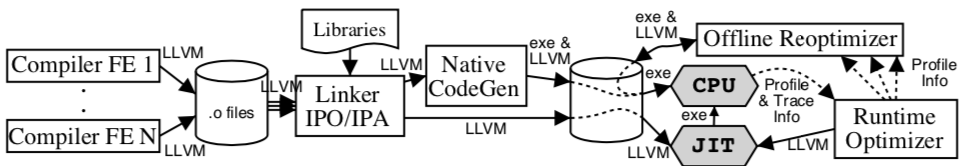
\includegraphics[width=\textwidth]{images/llvm-architecture.png}
    \caption{ The LLVM Compiler Framework Architecture \cite{lattner2004llvm}.}
    \label{fig:llvmarch}
    \Description[]{}
\end{figure*}
To achieve this ambitious goal, the framework utilizes a well defined, human-readable, intermediate representation called LLVM IR.
The IR, which is initially generated by the front end can be packaged with the target architecture binary along with profiling instructions for later runtime compilation (JIT) as well as more aggressive offline optimizations.
Several important characteristics of LLVM IR as as follows:
\begin{itemize}
    \item The IR maintains Static Single Assignment (SSA) form with unlimited virtual registers.
    \item Each register is of one of four primitive types: boolean, integer, floating-point or pointer.
    \item Similar to RISC, memory operations are carried out in registers, and between registers and memory using Load and Store instructions.
    \item The IR is limited to 31 opcodes.
    \item The IR is organized into basic blocks which must be composed into valid control flow graphs, simplifying the work required for various optimizations. 
\end{itemize}

\begin{lstlisting}[float,floatplacement=H,
caption={LLVM IR for a function multiplying x * y and adding z \cite{LLVM_Jit_Tutorial}},
label=lst:llvm_ir]
define i32 @mul_add(i32 %x, i32 %y, i32 %z) {
    entry:
    %tmp = mul i32 %x, %y
    %tmp2 = add i32 %tmp, %z
    ret i32 %tmp2
}\end{lstlisting}

This report will focus on LLVM's JIT component, which can be accessed through the MCJIT API.
The MCJIT framework provides an API thats accepts IR, generates optimized machine code, and provides a function pointer for calling the generated code.
The JIT compiler offers several levels of optimization: none, less, default, and aggressive, which correspond to O0-O3.
It should be noted that the JIT compiler by default does not perform any IR optimizations or transformations.
Instead, a developer must pass the generated IR to a Pass manager with specific optimizations.
This optimized IR can then be passed to the JIT Engine.

\section{JitBuilder}
\label{sec:jitbuilder}
JITBuilder.

\subsection{LLVM}
\label{sec:llvm}
LLVM, which at one time stood for Low-Level Virtual Machine, is a popular set of open-source, modular compiler and toolchain components \cite{lattner2004llvm}.
The compiler framework was originally designed to provide analysis and transformation for an application throughout its entire lifetime: from initial compilation and linking, through to runtime and even while the application was offline (see Figure \ref{fig:llvmarch}).
\begin{figure*}
    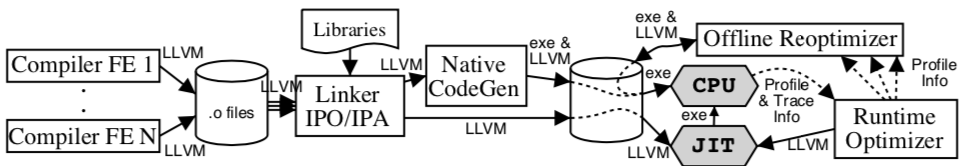
\includegraphics[width=\textwidth]{images/llvm-architecture.png}
    \caption{ The LLVM Compiler Framework Architecture \cite{lattner2004llvm}.}
    \label{fig:llvmarch}
    \Description[]{}
\end{figure*}
To achieve this ambitious goal, the framework utilizes a well defined, human-readable, intermediate representation (IR) called LLVM IR.
The IR, which is initially generated by the front end, can be packaged with the target architecture binary that includes profiling instructions for later runtime compilation (JIT) as well as more aggressive offline optimizations.
Several important characteristics of LLVM IR are as follows:
\begin{itemize}
    \item The IR maintains Static Single Assignment (SSA) form with unlimited virtual registers.
    \item Each register is of one of four primitive types: boolean, integer, floating-point or pointer.
    \item Similar to RISC, memory operations are carried out in registers, while operations between registers and memory use Load and Store instructions.
    \item The IR is limited to 31 opcodes.
    \item The IR is organized into basic blocks which must be composed into valid control flow graphs, simplifying the work required for various optimizations. 
\end{itemize}

\begin{lstlisting}[float,floatplacement=H,
caption={LLVM IR for a function returning x * y + z \cite{LLVM_Jit_Tutorial}.},
label=lst:llvm_ir]
define i32 @mul_add(i32 %x, i32 %y, i32 %z) {
    entry:
    %tmp = mul i32 %x, %y
    %tmp2 = add i32 %tmp, %z
    ret i32 %tmp2
}\end{lstlisting}

This report will focus on LLVM's JIT component, which can be accessed through the MCJIT application programming interface (API).
The MCJIT framework provides an API that accepts IR, generates optimized machine code, and provides a function pointer for calling the generated code.
The JIT compiler offers several levels of optimization: none, less, default, and aggressive.
It should be noted that the JIT compiler by default does not perform any IR optimizations or transformations.
Instead, a developer must pass the generated IR to a PassManager with specific optimizations they intend to apply.
These passes can be categorized as analysis passes, or transformation passes \cite{LLVM_Passes}:
\begin{itemize}
    \item Analysis Passes: collects information about IR for use later by transformations, for debugging or for visualization. 
    A few examples are \textit{print-callgraph}, \textit{print-function}, and \textit{iv-users} for printing the users of a particular induction variable. There are roughly 40 such passes available.
    \item Transformation Passes: These typically modify IR. Examples include \textit{adce} for dead code elimination, \textit{instcombine} for combining redundant instructions, or peephole optimizing, and \textit{tailcallelim} for eliminating tail calls. There are roughly 60 such passes available.
\end{itemize}
Generated IR can then be used by the ExecutionEngine to generate code for the target architecture.
Before a function is executed by the ExecutionEngine, it first checks if the code cache, or ObjectCache, contains a copy.
If the function could not be found, the compiler will generate the JIT code and store it in the ObjectCache before execution \cite{LLVM_MCJIT}.
It is worth noting that a newer JIT API, called ORCJIT, is also part of the LLVM project.
ORCJIT, or On-Request-Compilation JIT, is intended to complement the MCJIT API -- which compiles eagerly, by adding support for both lazy and concurrent compilations \cite{LLVM_ORCJIT}.

\subsection{JitBuilder}
\label{sec:jitbuilder}
JitBuilder is the embeddable framework for interacting with the Eclipse OMR JIT compiler Testarossa \cite{jitbuilderPaper}.
Eclipse OMR is an open-source collection of components for building language runtime environments.
Some of OMR's components include a garbage collection framework, a thread library, cross-platform port support, virtual machine building blocks, and a JIT compiler \cite{eclipseOMR,RebuildingAirliner}.
Much of the infrastructure driving Eclipse OpenJ9, a popular, open-source Java Virtual Machine, links to OMR components.

Through JitBuilder's API, users generate IR upon which optimizations are applied and from which native code is generated \cite{SuganumaIBMJit}.
Based on basic-blocks, the IR is arranged into directed acyclic graphic (DAG) structures called trees, composed of nodes which each contain an opcode.
OMR IR has several hundred opcodes, where typically with each type operation has a code for each data type: integer, pointer, double, float, vector, etc...\footnote{
    This can be contrasted with LLVM's roughly 31 opcodes, where the data type code is instead embedded within the instruction.
}
The children of these opcode nodes are in turn operands.
Trees with side-effects, which cannot be reordered, belong to a list of elements called treetops \cite{treetops}.
Existing nodes can be reused within a given tree, making optimizations such as common subexpression elimination relatively simple (see Listing \ref{lst:jitbuilder_ir}).
Though Testarossa supports several levels of optimization ranging from \textit{cold}, with roughly 20 optimizations applied, all the way to \textit{scorching}, where as many as 170 optimizations are applied, as of writing, JitBuilder is locked at the \textit{Warm} optimization level \cite{sanchez2011using, jitbuilderWarm}.
\begin{lstlisting}[float,floatplacement=H,
caption={OMR IR representation for (a+b)*(a-b). Note that the iload nodes are reused \cite{treetops}.},
label=lst:jitbuilder_ir]
treetop--> istore a
            |
            imul--- isub-------+
            |                  |
            iadd               |
            |                  |
            +-----> iload b <--+
            |                  |
            +-----> iload a <--+
}\end{lstlisting}



\section{Questions and Methods}
\label{sec:methodology}
To answer the questions we outlined in the introduction, we wrote three simple programs for both LLVM MCJIT and JitBuilder.
For the sake of comparison, we also wrote the programs using standard C++ without any JIT framework.
The programs are as follows:
\begin{itemize}
    \item increment - Calls a single function that adds one to an integer argument.
    \item recursive-fib - Calls a recursive Fibonacci function - \textit{fib(20)}. 
    \item iterative-fib - Calls an iterative Fibonacci function - \textit{fib(20}.  
\end{itemize}
For the JIT implementations, the IR was built using the provided APIs, then native code was generated and later used for the actual function calls.
We built and benchmarked the programs on an x86-64 Linux workstation running Ubuntu 19.04 with 32GB of RAM and an Intel i7-8700 (6-core, 12 thread) processor. 
Both LLVM and OMR were built from source code from their respective GitHub repositories \cite{llvmCommit, omrCommit}.
All the source code for this project can be found online\cite{projectGithub}.

\section{Results}
\label{sec:results}
\subsection{Compilation Time}
The first question we looked at was how long each framework took to compile a function. 
This time includes running the program from start to finish and includes the setup and teardown time of the JIT.
Each program was executed 20 times.

In Table \ref{tab:compile_time} we see that for the increment task JitBuilder compiled the function 61.5\% faster than MCJIT.
Looking into this further, the initial run to compile the function was roughly 900,000 nanoseconds.
Repeated executions made by our benchmarking framework\cite{googleBench} were closer to 500,000 nanoseconds as the instructions for this relatively small example were likely be cached.
For the other two tasks, we see that MCJIT was able to compile the functions more quickly than JitBuilder (recursive-fib compiled 16.5\% faster, and iterative-fib compiled 40.1\% faster ).


\begin{table*}[t]
  \begin{tabular}{|r|l|l|l|l|l|l|}
  \hline
  \multicolumn{1}{|l|}
  {\multirow{2}{*}{}} 
  & \multicolumn{3}{c|}{\textbf{LLVM MCJIT}}                                                                                                     & \multicolumn{3}{c|}{\textbf{Eclipse OMR JitBuilder}}                                                                              \\ \cline{2-7}
  
  \multicolumn{1}{|c|}{\textbf{Program}}
  & \multicolumn{1}{c|}{mean (ns)}  
  & \multicolumn{1}{c|}{median}  
  & \multicolumn{1}{c|}{std. dev.}     
  & \multicolumn{1}{c|}{mean (ns)}           
  & \multicolumn{1}{c|}{median} 
  & \multicolumn{1}{c|}{std. dev.}             
  \\ \hline
  
  increment                               
  & \num{1378060} %llvm                            
  & \num{1387338}                
  & \num{39774}               
  & \num{536741}  %jitbuilder                           
  & \num{537103}                
  & \num{2620}                                 
  \\ \hline
  
  recursive-fib                           
  & \num{1548316} %llvm                           
  & \num{1547491}                
  & \num{3925}                
  & \num{1854393} %jitbuilder                           
  & \num{1850322}               
  & \num{21754}
  \\ \hline
  
  iterative-fib                           
  & \num{2509502} %llvm                           
  & \num{2519808}                
  & \num{60429}              
  & \num{4192213} %jitbuilder                           
  & \num{4191730}               
  & \num{10419}                                
  \\ \hline
  
\end{tabular}
  \caption{Results of compiling each function 25 times with each JIT framework.}
  \label{tab:compile_time}
\end{table*}


% Increment IR generation for JitBuilder
\begin{lstlisting}[float,floatplacement=H,
  caption={Generating JitBuilder IR for the increment program.},
  label=lst:jitbuilder_increment]
bool IncrementMethod::buildIL()
{
  Return(
    Add(
        Load("value"),
        ConstInt32(1)));
  return true;
}
\end{lstlisting}

% IR code for LLVM increment
\begin{lstlisting}[float,floatplacement=H,
  caption={Generating MCJIT IR for the increment program.},
  label=lst:llvm_increment]
static Function *CreateIncrementFunction(
                  Module *M, 
                  LLVMContext &c) {
  FunctionType *f = FunctionType::get(Type::getInt32Ty(c), 
                      {Type::getInt32Ty(c)}, 
                      false);
  
  Function *incrementF = Function::Create(f, 
                      Function::ExternalLinkage, 
                      "increment", 
                      M);

  BasicBlock *BB = BasicBlock::Create(c, 
                      "EntryBlock", 
                      incrementF);
  
  Value *One = ConstantInt::get(Type::getInt32Ty(c), 1);
  
  Argument *ArgX = &*incrementF->arg_begin(); 
  ArgX->setName("AnArg");

  Value *Sum = BinaryOperator::CreateAdd(ArgX, 
                                One,
                                "addresult", 
                                BB);

  ReturnInst::Create(c, Sum, BB);
  return incrementF;
}
\end{lstlisting}

\subsection{Execution Time}
With JIT compilation completed, we turn to measuring how much CPU time is spent actually executing the function.
To measure this, we compiled the function once and then executed the compiled function 1000 times.
For each program, the process was repeated 20 times (see Table \ref{tab:1k_time_with_one_compile}).
Aside from the increment program, which favoured JitBuilder, both the recursive and iterative fib functions executed more quickly with LLVM generated code (0.53\% faster for recursive, and 0.37\% faster for iterative).
Compiling the test programs with GCC 5.3, having an optimization level of O3 (large binary, fast code), we saw extremely low execution times for the native increment program as our function calls were essentially optimized away.
It is worth noting that the code generated by the LLVM recursive-fib outperformed the native optimized code.
Given two of our programs performed more quickly with MCJIT than with JitBuilder, it is interesting to examine the disassembly of the generated code.\footnote{We used GDB to print instructions starting at the function pointer address. The disassembly is using Intel style.}

Examining the recursive-fib disassembly for JitBuilder (code listing \ref{lst:jitbuilder_rfib_assembly}), we see it is using the stack for storage. We expect these additional loads and stores, used for passing arguments and return values, are the reason for the performance disparity.
The LLVM disassembly (code listing \ref{lst:llvm_rfib_assembly}) on the other hand, passes arguments using registers.
It's also interesting to see the condition for the jump comparison: \texttt{jg} 0x2 with LLVM and \texttt{jl} 0x2 in JitBuilder. 
We would expect the latter to be the better optimization considering most times \texttt{n} is greater than 2.
The code in the LLVM listing would perform relative jumps more often, while the code in the JitBuilder would flow through the instructions more often.

Looking at the estimated execution time minus JIT compilation for 1000 functions calls (see Table \ref{tab:1k_executions}), we can see that JitBuilder's generated code outperformed MCJIT both in the iterative-fib programs.\footnote{In our tests, the compile time plus the execution time of the JIT-ed function was less than the measurement for just the compilation. As noted earlier, we suspect this performance has to do with a high degree of cache locality. We subtracted the mean from Table \ref{tab:compile_time} from the mean from Table \ref{tab:1k_time_with_one_compile} without accounting for the variance. This may be incorrect. Unfortunately, time constraints limited our ability to properly benchmark 1000 executions of the JIT-ed code.}


\begin{table*}[t]
  \begin{tabular}{|r|l|l|l|l|l|l|l|l|l|}
  \hline
  
  \multicolumn{1}{|l|}{\multirow{2}{*}{}} 
  & \multicolumn{3}{c|}{\textbf{LLVM MCJIT}}                                                                                    
  & \multicolumn{3}{c|}{\textbf{Eclipse OMR JitBuilder}}                                                                
  & \multicolumn{3}{c|}{\textbf{Native (C++)}}                                                                              
  \\ \cline{2-10}
  
  \multicolumn{1}{|c|}{\textbf{Program}}  
  & \multicolumn{1}{c|}{mean (ns)}  %llvm         
  & \multicolumn{1}{c|}{median}  
  & \multicolumn{1}{c|}{std. dev.}                     
  & \multicolumn{1}{c|}{mean (ns)}  %jb         
  & \multicolumn{1}{c|}{median}  
  & \multicolumn{1}{c|}{std. dev.}           
  & \multicolumn{1}{c|}{mean (ns)}  %native
  & \multicolumn{1}{c|}{median}  
  & \multicolumn{1}{c|}{std. dev.}                        
  \\ \hline
  
  increment                               
  & \num{1463310} %llvm
  & \num{1463032}                
  & \num{1660}                                        
  & \num{534192}  %jb                           
  & \num{534064}                 
  & \num{869}                                
  & \num{0.876}    %nat                          
  & \num{0.875}                   
  & \num{0.002}                                
  \\ \hline
  
  recursive-fib                           
  & \num{13674832}  %llvm                        
  & \num{13664199}               
  & \num{26548}                                        
  & \num{28707381}  %jb                         
  & \num{28699013}               
  & \num{29480}                               
  & \num{16016325}  %nat                        
  & \num{15996370}               
  & \num{60459}  
  \\ \hline
  
  iterative-fib                           
  & \num{2657528}   %llvm                         
  & \num{2668792}                
  & \num{83388}                                        
  & \num{4227967}   %jb                         
  & \num{4190232}                
  & \num{102744}                              
  & \num{0.876}     %nat                        
  & \num{0.875}                  
  & \num{0.003}                                
  \\ \hline
  \end{tabular}
  \caption{Results of JIT compiling each function once and executing the generated code 1000 times.}
  \label{tab:1k_time_with_one_compile}
\end{table*}

% Increment IR generation for JitBuilder
\begin{lstlisting}[float,floatplacement=H,
  caption={LLVM MCJIT recursive-fib disassembly (Optimization level 3)},
  label=lst:llvm_rfib_assembly]
(gdb) x/24i $1                                                              
  0x7ffff7fcd000 <fib>:        push   rbp                                  
  0x7ffff7fcd001 <fib+1>:      push   r14                                  
  0x7ffff7fcd003 <fib+3>:      push   rbx                                  
  0x7ffff7fcd004 <fib+4>:      cmp    edi,0x2                              
  0x7ffff7fcd007 <fib+7>:      jg     0x7ffff7fcd013 <fib+19>              
  0x7ffff7fcd009 <fib+9>:      mov    eax,0x1                              
  0x7ffff7fcd00e <fib+14>:     pop    rbx                                  
  0x7ffff7fcd00f <fib+15>:     pop    r14                                  
  0x7ffff7fcd011 <fib+17>:     pop    rbp                                  
  0x7ffff7fcd012 <fib+18>:     ret                                         
  0x7ffff7fcd013 <fib+19>:     mov    ebx,edi                              
  0x7ffff7fcd015 <fib+21>:     lea    edi,[rbx-0x1]                        
  0x7ffff7fcd018 <fib+24>:     movabs r14,0x7ffff7fcd000                   
  0x7ffff7fcd022 <fib+34>:     call   r14                                  
  0x7ffff7fcd025 <fib+37>:     mov    ebp,eax                              
  0x7ffff7fcd027 <fib+39>:     add    ebx,0xfffffffe                       
  0x7ffff7fcd02a <fib+42>:     mov    edi,ebx                              
  0x7ffff7fcd02c <fib+44>:     call   r14                                  
  0x7ffff7fcd02f <fib+47>:     add    eax,ebp                              
  0x7ffff7fcd031 <fib+49>:     pop    rbx                                  
  0x7ffff7fcd032 <fib+50>:     pop    r14                                  
  0x7ffff7fcd034 <fib+52>:     pop    rbp                                  
  0x7ffff7fcd035 <fib+53>:     ret    
\end{lstlisting}

\begin{lstlisting}[float,floatplacement=H,
caption={JitBuilder recursive-fib disassembly (Optimization level \textit{Warm})},
label=lst:jitbuilder_rfib_assembly]
(gdb) x/32i $1
  0x7ffff6a81034:	sub    rsp,0x18
  0x7ffff6a81038:	mov    QWORD PTR [rsp+0x10],rbx
  0x7ffff6a8103d:	cmp    edi,0x2
  0x7ffff6a81040:	jl     0x7ffff6a8106d
  0x7ffff6a81042:	mov    rbx,rdi
  0x7ffff6a81045:	lea    edi,[rbx-0x2]
  0x7ffff6a81048:	call   0x7ffff6a81034
  0x7ffff6a8104d:	mov    rdi,rbx
  0x7ffff6a81050:	mov    rbx,rax
  0x7ffff6a81053:	sub    edi,0x1
  0x7ffff6a81056:	call   0x7ffff6a81034
  0x7ffff6a8105b:	xchg   rbx,rax
  0x7ffff6a8105e:	mov    rcx,rbx
  0x7ffff6a81061:	add    eax,ecx
  0x7ffff6a81063:	mov    rbx,QWORD PTR [rsp+0x10]
  0x7ffff6a81068:	add    rsp,0x18
  0x7ffff6a8106c:	ret    
  0x7ffff6a8106d:	mov    rax,rdi
  0x7ffff6a81070:	mov    rbx,QWORD PTR [rsp+0x10]
  0x7ffff6a81075:	add    rsp,0x18
  0x7ffff6a81079:	ret   
\end{lstlisting}

\begin{table*}[t]
  \begin{tabular}{|r|l|l|} 
  \hline
  \multicolumn{1}{|c|}{\textbf{Program}}
  & \multicolumn{1}{c|}{\textbf{LLVM MCJIT}}                      
  & \multicolumn{1}{c|}{\textbf{Eclipse OMR JitBuilder}}
  \\ \hline

  increment                               
  & \multicolumn{1}{r|}{\num{85250}} %llvm      
  & \multicolumn{1}{r|}{\num{0}}     %jitbuilder               
  \\ \hline
  
  recursive-fib                           
  & \multicolumn{1}{r|}{\num{12126516}} %llvm       
  & \multicolumn{1}{r|}{\num{26852988}} %jitbuilder
  \\ \hline
  
  iterative-fib                           
  & \multicolumn{1}{r|}{\num{148026}} %llvm
  & \multicolumn{1}{r|}{\num{35754}} %jitbuilder
  \\ \hline
  
\end{tabular}
  \caption{Estimated time to execute JIT function 1000 times (mean from Table \ref{tab:1k_time_with_one_compile} - mean from Table \ref{tab:compile_time}). JitBuilder's increment score is listed as 0 because the compile and execution time was actually slightly lower than the compile time itself. We suspect these low values were due to a high degree of cache locality exhibited by the program.}
  \label{tab:1k_executions}
\end{table*}


\subsection{Binary File Size}
Looking at the size of the generated files (see Table \ref{tab:size_in_bytes}), the linked LLVM MCJIT programs are roughly six times larger in size than the JitBuilder programs.
Note that the JIT frameworks were compiled without debug symbols.
Part of the explanation for this is may have to do with over-linking the LLVM programs.
While there are over 167 possible linkable modules when using LLVM, I found the minimal set required to use MCJIT was just 8 : \textit{core, executionengine, interpreter, passes, mc, mcjit, support, nativecodegen}.

\begin{table*}[t]
  \begin{tabular}{|r|l|l|l|} 
  \hline
  \multicolumn{1}{|c|}{\textbf{Program}}
  & \multicolumn{1}{c|}{\textbf{LLVM MCJIT}}                      
  & \multicolumn{1}{c|}{\textbf{Eclipse OMR JitBuilder}}
  & \multicolumn{1}{c|}{\textbf{Native (C++)}}                    
  \\ \hline

  increment                               
  & \multicolumn{1}{r|}{\num{60640216}} %llvm      
  & \multicolumn{1}{r|}{\num{10148608}} %jitbuilder               
  & \multicolumn{1}{r|}{\num{16616}}    %native 
  \\ \hline
  
  recursive-fib                           
  & \multicolumn{1}{r|}{\num{60671176}} %llvm       
  & \multicolumn{1}{r|}{\num{10149272}} %jitbuilder
  & \multicolumn{1}{r|}{\num{16600}}   %native 
  \\ \hline
  
  iterative-fib                           
  & \multicolumn{1}{r|}{\num{60652728}} %llvm
  & \multicolumn{1}{r|}{\num{10149184}} %jitbuilder
  & \multicolumn{1}{r|}{\num{16600}}   %native 
  \\ \hline
  
\end{tabular}
  \caption{Total size in bytes of linked binary test programs.}
  \label{tab:size_in_bytes}
\end{table*}

\subsection{Resident State Set}
The resident state (RSS) set is amount of data loaded into RAM during execution at any one time.
To measure the maximum RSS, we used the \texttt{time} utility (\texttt{/usr/bin/time -v}) to collect this.
Looking at the results in Table \ref{tab:max_rss}, we see that LLVM consistently had the largest RSS.
The memory overhead required by LLVM is roughly 4.5 times larger than JitBuilder's requirement.
Looking at the number of times inactive pages were reclaimed during execution (minor page faults), we see that LLVM had roughly 4 times the number of inactive pages collected.

\begin{table*}[t]
  \begin{tabular}{|r|l|l|l|l|l|l|}
  \hline
  
  \multicolumn{1}{|l|}{\multirow{2}{*}{}} 
  & \multicolumn{2}{c|}{\textbf{LLVM MCJIT}}                                                                                    
  & \multicolumn{2}{c|}{\textbf{Eclipse OMR JitBuilder}}                                                                
  & \multicolumn{2}{c|}{\textbf{Native (C++)}}                                                                              
  \\ \cline{2-7}
  
  \multicolumn{1}{|c|}{\textbf{Program}}  
  & \multicolumn{1}{c|}{max RSS (kb)}  %llvm         
  & \multicolumn{1}{c|}{minor page faults}  
  & \multicolumn{1}{c|}{max RSS (kb)}  %jb         
  & \multicolumn{1}{c|}{minor page faults}  
  & \multicolumn{1}{c|}{max RSS (kb)}  %native         
  & \multicolumn{1}{c|}{minor page faults}  
  \\ \hline

  increment                               
  & \multicolumn{1}{r|}{\num{43544}} %llvm  
  & \multicolumn{1}{r|}{\num{1478}} 
  & \multicolumn{1}{r|}{\num{9416}} %jitbuilder               
  & \multicolumn{1}{r|}{\num{344}}
  & \multicolumn{1}{r|}{\num{1548}}    %native 
  & \multicolumn{1}{r|}{\num{65}}
  \\ \hline
  
  recursive-fib                           
  & \multicolumn{1}{r|}{\num{45472}} %llvm       
  & \multicolumn{1}{r|}{\num{1545}} 
  & \multicolumn{1}{r|}{\num{9768}} %jitbuilder
  & \multicolumn{1}{r|}{\num{384}} 
  & \multicolumn{1}{r|}{\num{1532}}   %native 
  & \multicolumn{1}{r|}{\num{63}} 
  \\ \hline
  
  iterative-fib                           
  & \multicolumn{1}{r|}{\num{44452}} %llvm
  & \multicolumn{1}{r|}{\num{1520}}
  & \multicolumn{1}{r|}{\num{10044}} %jitbuilder
  & \multicolumn{1}{r|}{\num{423}}
  & \multicolumn{1}{r|}{\num{1684}}   %native 
  & \multicolumn{1}{r|}{\num{66}}  
  \\ \hline
  
\end{tabular}
  \caption{Maximum resident state set (RSS) in kilobytes during execution of a single compilation and execution of the generated function. Note that Native had no run-time compilation phase. A minor page fault occurs when the OS reclaims inactive pages during execution. Page size was 4096 bytes.}
  \label{tab:max_rss}
\end{table*}

\subsection{Developer Experience}
One additional aspect to overhead worth considering is the usability of the frameworks from a developer's perspective.
Under this banner, we looked at two items: ease of use, and how configurable the frameworks were.

\subsubsection{Usability}
While ease of use is not likely to be the highest priority when considering which JIT framework to select, research has shown that improved API usability can positively impact developer productivity \cite{apiUsability}, while improving code quality and reducing errors.
Overall we found that JitBuilder took less time to integrate, and provided a more intuitive API for generating IR.
When considering usability we took note of the following items:
\begin{itemize}
  \item Both of the frameworks provide public Github repositories \cite{llvmGithub,jitbuilderGithub}.
  \item The instructions for building the frameworks were readily available and simple to follow.
  \item Linking LLVM took considerable effort as it was unclear which of the 167 objects were required to use MCJIT. After some trial and error, we discovered LLVM provides a utility, \texttt{llvmconfig}, which simplifies this task by generating header and linking arguments for G++ based on a list of objects\footnote{Example commands for building the programs can be found \texttt{makefiles} in the accompanying source code \cite{projectGithub} under \texttt{src/<framework>/}.} 
  \item JitBuilder on the other hand required was simple to integrate, requiring only a single header file and single module to link: \texttt{jitbuilder}. On the other hand, LLVM required us to include 20 header files in our programs.
  \item We found that writing the IR generators in our test programs took less time with JitBuilder than with LLVM. 
  The most challenging task was writing iterative-fib for LLVM, as this required us to grasp the underlying IR requirements which included: an induction value, a Phi node, several basic blocks for before, during and after the loop, condition values, as well as allocation and store pointers.\footnote{Source code for the LLVM iterative-fibonacci program can be found in the CreateFibFunction within \texttt{src/llvm/iterative-fib/fib.cpp}}.
  \item We noticed that the number of lines of code to generate IR are typically fewer for JitBuilder. 
  This can be seen in the increment code listing for JitBuilder\ref{lst:jitbuilder_ir}, and for LLVM MCJIT\ref{lst:llvm_ir}.
  \item The in memory objects generated by LLVM MCJIT can contain debug symbols (DWARF format) allowing debugging to take place in GDB 7.0 and higher \cite{llvmDebugJIT}.
\end{itemize}

\subsubsection{Configuration}
While the API of LLVM MCJIT may have an overabundance of controls, it does provide an high level of configuration compared to JitBuilder, including which optimization and analysis passes to run, control over the memory structure of the generated code, control over the object cache, and what level of optimization to generate the code at.
As mentioned, JitBuilder on the other hand is currently locked at the \textit{Warm} optimization level, limiting the number of optimizations performed on the IR.


\section{Related Work}
\label{sec:related-work}
Given the overhead involved in fetching, decoding, and executing instructions, interpreters are a commonplace we see JIT compilers employed.
Java Virtual Machines \cite{HiPerfJava,SuganumaIBMJit} have been employing JIT compilers for over two decades, while the Python world has both
Numba, a Python JIT compiler based on LLVM \cite{numba,numbaWeb}, and the PyPy project -- a Python interpreter with its own tracing JIT \cite{pypy}.

JitBuilder has been integrated into several demonstration interpreters \cite{lua-vermhela, wasmjit, base9}, while work is ongoing to build new runtimes or to bolster existing runtimes with its parent project, Eclipse ORM \cite{ruby-omr}.

There is also work being done to allow JitBuilder to ingest LLVM IR \cite{llvm-jitbuilder-interop}. 
Not only would this allow JitBuilder to bolt onto existing LLVM based projects, but it could also help provide deeper insight into the quality and differences of the generated code between the two frameworks.







\section{Future Work}
\label{sec:future-work}
The number of test programs could be expanded to cover such scenarios as arrays, large vector operations, and very large functions.
In all the test examples, each JIT compilation required a complete teardown of the JIT infrastructure. 
It would be interesting to compare the performance of repeated JIT compilations.
While the JIT compiler in Eclipse OMR, TRJIT, supports many levels of compilation, as well as support for synchronous, and asynchronous compilation schemes, these options have not yet been exposed to JitBuilder.
JitBuilder could be expanded upon to provide such controls, though special attention would have to be given to the maintaining the usability of the API.
Finally, testing the compilers under more complex scenarios such as making JIT-to-JIT function calls, and dealing with code cache limitations would provide more realistic data.

\section{Summary}
\label{sec:summary}
Summary

\section{Acknowledgements}

This research was conducted within the Centre for Advanced Stu-\\dies---Atlantic, Faculty of Computer Science, University of New Brunswick. The authors are grateful for the colleagues and facilities of CAS Atlantic in supporting our research. The authors would like to acknowledge the funding support provided by the Atlantic Canada Opportunities Agency (ACOA) through the Atlantic Innovation Fund (AIF) program. Furthermore, we would also like to thank the New Brunswick Innovation Foundation for contributing to this project.

\bibliographystyle{unsrt}
\bibliography{refs}{}

\end{document}
\endinput
%%
%% End of file `paper.tex'.
